\documentclass[12pt,a4paper,english]{article}
\usepackage{times}
\usepackage[utf8]{inputenc}
\usepackage{babel,textcomp}
\usepackage{mathpazo}
\usepackage{mathtools}
\usepackage{amsmath,amssymb}
\usepackage{ dsfont }
\usepackage{listings}
\usepackage{graphicx}
\usepackage{ mathrsfs }
\usepackage{float}
\usepackage{subfig} 
\usepackage{multirow}
\usepackage[hyphens]{url}
\usepackage[colorlinks]{hyperref}
\hypersetup{breaklinks=true}
\usepackage[usenames,dvipsnames,svgnames,table]{xcolor}
\usepackage{textcomp}
\definecolor{listinggray}{gray}{0.9}
\definecolor{lbcolor}{rgb}{0.9,0.9,0.9}
\lstset{backgroundcolor=\color{lbcolor},tabsize=4,rulecolor=,language=python,basicstyle=\scriptsize,upquote=true,aboveskip={1.5\baselineskip},columns=fixed,numbers=left,showstringspaces=false,extendedchars=true,breaklines=true,
prebreak=\raisebox{0ex}[0ex][0ex]{\ensuremath{\hookleftarrow}},frame=single,showtabs=false,showspaces=false,showstringspaces=false,identifierstyle=\ttfamily,keywordstyle=\color[rgb]{0,0,1},commentstyle=\color[rgb]{0.133,0.545,0.133},stringstyle=\color[rgb]{0.627,0.126,0.941},literate={å}{{\r a}}1 {Å}{{\r A}}1 {ø}{{\o}}1}

% Use for references
\usepackage[square,comma,numbers]{natbib}
%\DeclareRobustCommand{\citeext}[1]{\citeauthor{#1}~\cite{#1}}

% Fix spacing in tables and figures
%\usepackage[belowskip=-8pt,aboveskip=5pt]{caption}
%\setlength{\intextsep}{10pt plus 2pt minus 2pt}

% Change the page layout
%\usepackage[showframe]{geometry}
%\usepackage{layout}
\setlength{\hoffset}{-0.7in}  % Length left
\setlength{\voffset}{-0.7in}  % Length on top
\setlength{\textwidth}{480pt}  % Width /597pt
\setlength{\textheight}{665pt}  % Height /845pt
%\setlength{\footskip}{25pt}

\newcommand{\VEV}[1]{\langle#1\rangle}
\title{FYS4411 - Project 1}
\date{}
\author{ Kristoffer Langstad \footnote{\url{https://github.com/krilangs/FYS4411/tree/master/Project1} \cite{GitHub}}\\ \textit{krilangs@uio.no}}

\begin{document}%\layout
\maketitle
\begin{abstract}
In this project we will build a variational Monte Carlo (VMC) method to evaluate the ground state energy of a trapped, hard sphere Bose gas for different numbers of particles in one, two and three dimensions with a specific trial wave function. We study non-interacting and interacting bosons in both spherical and elliptical harmonic oscillator potential traps. This is done by implementing both a more brute force Metropolis sampling and a more improved Metropolis-Hastings (Importance) sampling. The trial wave function consists of a single-particle Gaussian function and the hard-sphere Jastrow factor. The ground state energies are simulated from both an analytically derived expression and a numerically derived kinetic energy. These computed energies are compare to the Gross-Pitaevskii equation \cite{nilsen2005vortices}.

For non-interacting bosons the analytical derivation with the brute Metropolis is found the give the fastest CPU time and best results for the ground state energies. The interaction between the bosons increased the energy in the system as well as the optimal variational parameter $\alpha$. For the analytical case this optimal parameter was found to be $\alpha=0.5$, since this gave us the ground state energy of the system. For the interaction we used gradient descent to find the optimal parameter to be $\alpha=0.503275$ for 10 particles in 3D, which increased  as the number of particles in the system increased (still around 0.5). The clocking method, improved by \citet{jonsson2018standard}, was used to improve the numerical error in the energies to make it more realistic with correlation between the numerical data. The one-body density was also studied in case of the Jastrow factor importance on the system. This factor was found to give an interaction between the bosons that made the most probable distance between the bosons larger.
\end{abstract}

\section{Introduction}
\label{sect:Introduction}
A more and more interesting theme in physics is to look at confined Bose systems. Systems like this contains gases of alkali atoms which are confined in magnetic traps which givens dilute systems. In such systems, we can study the Bose-Einstein condensation (BEC) when bosons are cooled down to a critical temperature. At this critical temperature, the bosons will condense into the system ground state. There we can study the ground state energy with a specific wave function. Most studies of the BEC confined in magnetic or optical traps have been conducted in the framework of the Gross-Pitaevskii (GP) equation \cite{nilsen2005vortices}.

In this project we will study two cases, one where the bosons don't interact with each other and one where they interact as if they had hard shells. For both cases we will study systems in one, two and three dimensions with a varying number of particles in the system. Since we are looking at bosons in the ground state of the system, we can derive the ground state energy analytically. Here the analytical expression is quite simple for non-interacting bosons. In the interacting case we need also a correlation wave function term which is not needed for non-interacting bosons. This will complicate the expression for the local energy. For the traps we will use spherical and elliptical harmonic traps. The calculated local energies for the systems we look at can also be calculated with the GP equation which we will use as a benchmark for our numerically calculated energies.

To do the ground state energy calculation for this many-body system, for both system cases, we will use Variational Monte Carlo (VMC) methods in C++ with both a "brute force" Metropolis and a more improved Metropolis-Hastings algorithm, also called Importance sampling, and with a specific trial wave function. In this project we will use a single variational parameter $\alpha$. The optimal value of this variational parameter is found by implementing a gradient descent method for minimizing the ground state energy. With this optimal variational parameter we do a statistical analysis of the numerical data by using the blocking method to get a proper error analysis. Another thing we look at is the one-body density of the system where we study the correlation and importance of the Jastrow factor.

First we will look at the theory of the physics and the numerics we will use in this project. This includes an overview of among others the system, the analytical derivations of the local energy for both non-interacting and interacting cases, the Gross-Pitaevskii equation, one-body density and then the theory of the numerical methods mentioned above. In the methods section we explain what we do with the implementation of the numerical tools we are to use and what the parameters we are going to use are. It is here we do all the local energy sampling with the different interaction and non-interaction cases with brute force Metropolis and Importance sampling, as well as other studies of the systems. We will also benchmark our calculated ground state energies to the energies calculated with the GP equation. In the results section we will present and discuss all the results we get through this project. Lastly, we come up with a conclusion to the project with possible aspects towards future work.

\section{Theory}
\label{sect:Theory}
\subsection{The System}
\label{subsect:System}
We will consider a system of N bosons with masses $m$ which are trapped in a harmonic oscillator potential. For the alkali gas $^{87}$Rb, the characteristic dimensions/length of the trap is $a_{ho}=(\hbar/m\omega_{\perp})^{\frac{1}{2}}=1-2\times10^4$Å. For low energies it is sufficient enough to look at the s-wave scattering length $a_{Rb}$ which is often selected as $a_{Rb}=100a_0$, where $a_0=0.5292$Å is the Bohr radius. In \citet{dubois2001bose} they derive that both the trap size and the inter-atom spacing is much larger than the effective atom size leading to the condition for the system to be dilute. This leads to the system being dominated by two-body collisions. This gives that the system has the following two-body Hamiltonian
\begin{equation}
\label{eq:sys_Hamiltonian}
H=\sum_i^N\left(\frac{-\hbar^2}{2m}\nabla_i^2+V_{\text{ext}}(\textbf{r}_i)\right)+\sum_{i<j}^{N}V_{\text{int}}(\textbf{r}_i,\textbf{r}_j),
\end{equation}
which is going to work on a trial wave function $\Psi_T(\textbf{r})$. We will look at both a spherical (S) and an elliptical (E) harmonic trap up till three dimensions. They are modeled as a hard-shell models. The $V_{\text{ext}}(\textbf{r}_i)$ term is the harmonic oscillator potential, which in three dimensions is given by
\begin{equation}
\label{eq:V_ext}
V_{\text{ext}}(\textbf{r})= \Bigg\{
\begin{array}{ll}
\frac{1}{2}m\omega_{ho}^2r^2 & (S)\\
\strut
\frac{1}{2}m[\omega_{ho}^2(x^2+y^2) + \omega_z^2z^2] & (E)
\end{array}.
\end{equation}
Here $\omega_{ho}^2$ is the trap potential strength. For elliptical trap, $\omega_{ho}=\omega_{\perp}$ is the trap frequency in the perpendicular plane, while $\omega_z$ is the frequency in the z-direction. The ratio of the frequencies is denoted as $\lambda=\omega_z/\omega_{\perp}$ giving the ratio of the trap lengths 
\begin{equation*}
\frac{a_{\perp}}{a_z}=\left(\frac{\omega_z}{\omega_{\perp}}\right)^{\frac{1}{2}}=\sqrt{\lambda}.
\end{equation*} 
The $V_{\text{int}}(r_{ij})$ term is the hard-shell interaction potential given as
\begin{equation}
\label{eq:V_int}
V_{\text{int}}(r_{ij})= \Bigg\{
\begin{array}{ll}
\infty & |\textbf{r}_i-\textbf{r}_j|\leq a\\
\strut
0 & |\textbf{r}_i-\textbf{r}_j|> a
\end{array},
\end{equation}
with $r_{ij}=|\textbf{r}_i-\textbf{r}_j|$ is the distance between particle $i$ and $j$, and $a$ is the so-called hard-core diameter of the bosons.

For the ground state with N particles we will us the trial wave function
\begin{equation}
\label{eq:WF_T}
 \Psi_T(\mathbf{r})=\Psi_T(\mathbf{r}_1, \mathbf{r}_2, \dots \mathbf{r}_N,\alpha,\beta)
=\left[
\prod_i g(\alpha,\beta,\mathbf{r}_i)
\right]
\left[
\prod_{j<k}f(a,|\mathbf{r}_j-\mathbf{r}_k|)
\right], 
\end{equation}
where $\alpha$ and $\beta$ are variational parameters. We will use $\alpha$ as the only variational parameter, and treat $\beta$ as a constant to be chanegd according to if we have a spherical trap ($\beta=1$) or an elliptical trap ($\beta=2.82843$). The first part of the trial wave function (\ref{eq:WF_T}) is the one body harmonic oscillator ground state wave function, also called the Slater permanent,
\begin{equation}
\label{eq:g}
g(\alpha,\beta,\mathbf{r}_i)= e^{-\alpha(x_i^2+y_i^2+\beta z_i^2)},
\end{equation} 
and the second part is the correlation wave function, also called the Jastrow factor. For spherical traps and non-interaction bosons ($a=0$) we get $\alpha=\frac{1}{2a_{ho}^2}$ the correlation term yields
\begin{equation}
\label{eq:Jastrow}
J(\textbf{r})=f(a,\mathbf{r}_i,\mathbf{r}_j)=\Bigg\{
\begin{array}{ll}
0 & {|\mathbf{r}_i-\mathbf{r}_j|} \leq {a}\\
(1-\frac{a}{|\mathbf{r}_i-\mathbf{r}_j|}) & {|\mathbf{r}_i-\mathbf{r}_j|} > {a}.
\end{array}
\end{equation}
When scaling and using natural units later in this project, $\hbar=\omega=m=1$, we get $a_{ho}=1$ (as can be seen easily above) which then gives $\alpha=0.5$ for the ground state.

\subsection{Local Energy}
\label{subsect:Energy}
In this project, the quantity we will mostly be looking at is the local energy of the system defined as
\begin{equation}
\label{eq:local_energy}
E_L(\mathbf{r})=\frac{1}{\Psi_T(\mathbf{r})}H\Psi_T(\mathbf{r}).
\end{equation}  
The calculation of the energy of the system is done by computing the expectation value of the local energy:
\begin{equation}
\label{eq:expec_E}
\langle E_L\rangle=\langle H\rangle=\frac{\int E_L(\textbf{r})|\Psi_T(\textbf{r})|^2d\textbf{r}}{\int|\Psi_T(\textbf{r})|^2d\textbf{r}}\approx\frac{1}{N}\sum_{i=1}^{N}E_L(\textbf{r}_i)|\psi(\textbf{r}_i)|^2
\end{equation} 
$|\psi(\textbf{r})|^2$ is the probability density function. The ground state energy is where we have the minimum of the expectation value of the energy. To determine this we also calculate the variance 
\begin{equation}
\label{eq:variance}
\sigma^2=\langle E_L^2\rangle-\langle E_L\rangle^2,
\end{equation}
and the standard deviation $\sigma$. We want the variance to be as small as possible.

To compute the local energy we will find analytical expressions and compare it with numerically calculated energies of the system. Here we expect the analytical expression to be much more CPU friendly.

\subsection{Drift Force}
\label{subsect:F}
Since the brute force Metropolis-Hastings algorithm might use more time than needed at unwanted places, we want improve how the algorithm makes moves. In other words, we want to increase the acceptance rate of the proposed moves in the algorithm. So we introduce Importance sampling with a drift/quantum force $F(\textbf{r})$. The drift force is derived from the Fokker-Planck equation:
\begin{equation}
\label{eq:Fokker-Planck}
\frac{\partial P(\textbf{r},t)}{\partial t}=\sum_{k}D\left(\nabla_k^2\cdot P(\textbf{r},t)-D\nabla_k\cdot F(\textbf{r}_k)P(\textbf{r},t)\right)=\sum_{k}D\nabla_k\cdot(\nabla_k-F(\textbf{r}_k))P(\textbf{r},t)
\end{equation}
The first part is the standard diffusion equation with a diffusion coefficient $D$, and $P(\textbf{r},t)$ is a time-dependent probability density. We want a convergence to a stationary state with
\begin{align*}
\frac{\partial P}{\partial t}=0.
\end{align*}
This is only true if
\begin{align*}
\nabla_k^2 P=P\nabla_k \textbf{F}_k+\textbf{F}_k\nabla_k P.
\end{align*}
With the assumption of stationary densities:
\begin{align*}
\textbf{F}&=g(\textbf{r})\nabla P\\
\Rightarrow\quad \nabla_k^2 P&=P\nabla_k g\cdot(\nabla_k P)^2+Pg\nabla_k^2 P+g(\nabla_k P)^2
\end{align*}
The terms containing first and second derivatives have to cancel each other, which only happens if $g=\frac{1}{P}$. For a system with bosons the trial wave function is the probability density function and $D=1/2$ comes from the half factor in the kinetic energy (natural units). This yields the drift force for a single article $k$:
\begin{equation}
\label{eq:F}
F_k(\textbf{r})=\frac{2\nabla_k\Psi_T(\textbf{r})}{\Psi_T(\textbf{r})}
\end{equation}
This force will push the proposed moves towards the regions of configuration space where the trial wave function is large, which should increase the acceptance rate of the moves made.

\subsection{The Gross-Pitaevskii equation}
\label{subsect:GP_eq}
In this project we look at alkali gases which are diluted. This means that they can be computed using the mean field Gross-Pitaevskii (GP) equation. The GP equation in \citet{dubois2001bose} is defined as
\begin{equation}
\label{eq:GP_eq}
E_{GP}[\Psi]=\int d\textbf{r}\left[\frac{\hbar^2}{2m}|\nabla\Psi(\textbf{r})|^2+V_{\text{trap}}(\textbf{r})|\Psi|^2+\frac{2\pi\hbar^2a}{m}|\Psi|^4\right],
\end{equation}
where $V_{\text{trap}}(\textbf{r})=\frac{1}{2}m(\omega_{\perp}^2x^2+\omega_{\perp}^2y^2+\omega_z^2z^2)$ is the three dimensional elliptical harmonic potential. The generalized derivation of this equation can be seen in Appendix \ref{appendix:GP_eq}. This is generalized to work for one, two and three dimensions as
\begin{equation}
\label{eq:GP_derived}
E_{GP}[\Psi_T]=\frac{N}{2}\frac{d}{3}\left(\alpha+\frac{1}{4\alpha}\right)(\beta+2)
\end{equation}
This equation (\ref{eq:GP_derived}) is the benchmark energy to be used for comparison to the computed local energy for spherical and elliptical harmonic oscillator traps in $d$ dimensions for N particles later in the project.

\subsection{Non-Interacting Bosons}
\label{subsect:non-int}
\subsubsection{Drift Force and Local Energy Analytical}
\label{subsubsect:EL_analytic}
For non-interacting bosons in a spherical trap with $a=0$ and $\beta=1$, the correlation term in the trial wave function (eq. \ref{eq:WF_T}) vanishes:
\begin{equation}
\label{eq:nonint_WF_T}
\Psi_T(\textbf{r})=\prod_i g(\alpha,1,\mathbf{r}_i)=\prod_{i}e^{-\alpha(x_i^2+y_i^2+z_i^2)}=\prod_{i}e^{-\alpha|\textbf{r}_i|^2}
\end{equation}
In this case it is easy to switch between the number of dimensions since 1D: $\textbf{r}_i^2=x_i^2$, 2D: $\textbf{r}_i^2=x_i^2+y_i^2$ and 3D: $\textbf{r}_i^2=x_i^2+y_i^2+z_i^2$.

Since $a=0$ the interaction potential $V_{\text{int}}(\textbf{r}_{ij})$ (eq. \ref{eq:V_int}) also vanishes, and we get the spherical term of the harmonic potential $V_{\text{ext}}(\textbf{r})$ (eq. \ref{eq:V_ext}). This then gives the new Hamiltonian as
\begin{equation}
\label{eq:non-int_H}
H=\sum_{i=1}^N\left(\frac{-\hbar^2}{2m}\nabla_i^2+\frac{1}{2}m\omega_{ho}^2r_i^2\right).
\end{equation}
We now have the trial wave function and the Hamiltonian needed for the local energy in equation \ref{eq:local_energy}. The next thing we have to compute is the gradient ($\nabla$) and the Laplacian ($\nabla^2$) of the trial wave function. The gradient for a particle $k$ of equation \ref{eq:nonint_WF_T} is
\begin{equation}
\label{eq:grad_WF_T}
\nabla_k\Psi_T(\textbf{r})=-2\alpha \textbf{r}_ke^{-\alpha|\textbf{r}_k|^2}=-2\alpha \textbf{r}_k\Psi_T(\textbf{r}).
\end{equation} 
The Laplacian is then
\begin{equation}
\label{eq:Laplacian_WF_T}
\nabla_k^2\Psi_T(\textbf{r})=(-2\alpha d+4\alpha^2r_k^2)e^{-\alpha|\textbf{r}_k|^2}=(-2\alpha d+4\alpha^2r_k^2)\Psi_T(\textbf{r}),
\end{equation}
with dimensionality $d$ of the system.

For a particle $k$ we can use the gradient of the trial wave function (eq. \ref{eq:grad_WF_T}) to find the drift force from equation \ref{eq:F}:
\begin{equation}
\label{eq:Drift_F_nonint}
F_k(\textbf{r})=\frac{2}{\Psi_T(\textbf{r})}(-2\alpha \textbf{r}_k)\Psi_T(\textbf{r})=-4\alpha\textbf{r}_k
\end{equation}

With the Laplacian of the trial wave function in equation \ref{eq:Laplacian_WF_T} we can compute the non-interacting Hamiltonian in equation \ref{eq:non-int_H} and then the local energy in equation \ref{eq:local_energy}:
\begin{align*}
E_L(\textbf{r})&=\frac{1}{\Psi_T(\textbf{r})}\sum_{i=1}^{N}\left(\frac{-\hbar^2}{2m}(-2\alpha d+4\alpha^2r_i^2)\Psi_T(\textbf{r})+\frac{1}{2}m\omega_{ho}^2r_i^2\Psi_T(\textbf{r})\right)\nonumber\\
&=\sum_{i=1}^{N}\left(\frac{-\hbar^2}{2m}(-2\alpha d+4\alpha^2r_i^2)+\frac{1}{2}m\omega_{ho}^2r_i^2\right)
\end{align*}
Since we will use scaling and natural units, $\hbar=m=c=1$ and use $\omega_{ho}=1$, we can simplify the local energy to
\begin{equation}
\label{eq:local_E_nonint}
E_L(\textbf{r})=\alpha dN+(-2\alpha^2+\frac{1}{2})\sum_{i=1}^{N}r_i^2.
\end{equation}
If we choose $\alpha=0.5$; 
\begin{equation}
\label{eq:local_E_stable}
E_L(\textbf{r};\alpha=0.5)=\frac{dN}{2},
\end{equation}
we see that the local energy becomes stable depending on the dimensionality of the system and the number of particles. This will give the ground state energy of the system in this case. In appendix \ref{appendix:Optimal_alpha} we derive another way to show that $\alpha=0.5$ is the optimal variational parameter in this case.

\subsubsection{Local Energy Numerical}
\label{subsubsect:EL_num}
We will also in this non-interacting case compute the local energy numerically. Here we calculate the kinetic and potential energy and sum them up. With scaling, natural units and oscillator frequency $\omega=\omega_{ho}$:
\begin{equation}
\label{eq:local_E_num}
E_L=E_k+E_p=-\frac{1}{2}\frac{1}{\Psi_T}\sum_i^{N}\nabla_i^2\Psi_T+\frac{1}{2}\sum_{i=1}^{N}\omega^2r_i^2
\end{equation}
To solve this system numerically we use the Forward Euler finite difference approximation method, with time step $h$, for each dimension (x, y, z):
\begin{equation*}
\nabla^2 u\approx \frac{u(i+h)-2u(i)+u(i-h)}{h^2},\quad i=0,1,...,N
\end{equation*}

\subsection{Interacting Bosons}
\label{subsect:interact}
\subsubsection{Drift Force and Local Energy}
\label{subsubsect:local_E_int}
For the more realistic system we look at interacting bosons in the potential trap. For the interacting elliptical system $a\neq0$ and $\beta\neq0$. Now we have the full trial wave function in equation \ref{eq:WF_T}. Then we change the Slater permanent (eq. \ref{eq:g}) as $g(\alpha,\beta,\mathbf{r}_i)=\phi(\textbf{r}_i)$, and the Jastrow factor (eq. \ref{eq:Jastrow}) as 
\[\prod_{j<k}f(r_{jk})=\exp\left(\sum_{j<k}u(r_{jk})\right)\]
with $r_{jk}=|\textbf{r}_j-\textbf{r}_k|$ and $u(r_{jk})=\ln f(r_{jk})$. The final expression for the trial wave function is then
\begin{equation}
\label{eq:WF_T_int}
\Psi_T(\mathbf{r})=\left[\prod_i \phi(\textbf{r}_i)\right]
\exp\left(\sum_{j<k}u(r_{jk})\right).
\end{equation}

To find the drift force (eq. \ref{eq:F}) for particle $k$ in the interacting case, we take the gradient of this new trial wave function (also used in the Laplacian later). This gradient is derived in Appendix \ref{appendix:Laplacian}. The drift force for particle $k$ with the gradient of the trial wave function in this appendix then becomes:
\begin{align}
\label{eq:drift_force_int}
F_k({\textbf{r}})&=\frac{2}{\Psi_T(\textbf{r})}\left(\frac{\nabla_k\phi(\textbf{r}_k)}{\phi(\textbf{r}_k)}+\sum_{l\neq k}\nabla_k u(r_{kl})\right)\Psi_T(\textbf{r})\nonumber\\
&=2\left(\frac{\nabla_k\phi(\textbf{r}_k)}{\phi(\textbf{r}_k)}+\sum_{l\neq k}\nabla_k u(r_{kl})\right)
\end{align}

The next thing needed again is to compute the second derivative in the full Hamiltonian (eq. \ref{eq:sys_Hamiltonian}). The Laplacian divided by the trial wave function becomes:
\begin{align}
\label{eq:Laplacian_int}
\frac{\nabla_k^2\Psi_T(\textbf{r})}{\Psi_T(\textbf{r})}&= \frac{\nabla_k^2\phi(\textbf{r}_k)}{\phi(\textbf{r}_k)}+2\frac{\nabla_k\phi(\textbf{r}_k)}{\phi(\textbf{r}_k)}\left(\sum_{j\neq k}u^{\prime}(r_{kj})\frac{\Delta\textbf{r}_{kj}}{r_{kj}}\right)+\sum_{i,j\neq k}\frac{\Delta \textbf{r}_{ki}\Delta \textbf{r}_{kj}}{r_{ki}r_{kj}}u^{\prime}(r_{ki})u^{\prime}(r_{kj})\nonumber\\
&+\sum_{j\neq k}\left(u^{\prime\prime}(r_{kj})+\frac{d-1}{r_{kj}}u^{\prime}(r_{kj})\right)
\end{align}
The full derivation of this equation can be seen in Appendix \ref{appendix:Laplacian}, and $d$ is the dimensionality of the system. 
Inserting all the derived equations in Appendix \ref{appendix:Laplacian} with the Hamiltonian for interacting bosons (eq. \ref{eq:sys_Hamiltonian}) into the local energy (eq. \ref{eq:local_energy}), we get (full derivation in Appendix \ref{appendix:local_E}):
\begin{align}
\label{eq:local_E_full}
E_L(\textbf{r})=-\frac{\hbar^2}{2m}\sum_k^N\frac{\nabla_k^2\Psi_T(\textbf{r})}{\Psi_T(\textbf{r})}
+\frac{1}{2}m\sum_k^N[\omega^2(x_k^2+y_k^2) + \omega_z^2z_k^2]
+\sum_{j<k}^{N}V_{\text{int}}(\textbf{r}_j,\textbf{r}_k)
\end{align}
Insert the Laplacian divided by the trial wave function in equation \ref{eq:H_int_deriv} into the local energy above for full expression. We do not write the full expression since the equation becomes so large.

\subsubsection{Scaling}
\label{subsubsect:Scaling}
For the elliptic trap with a repulsive interaction we introduce energy in units of $\hbar\omega_{ho}$ and lengths in units of $a_{ho}=\sqrt{\frac{\hbar}{m\omega_{ho}}}=(1-2)\times10^4$Å such that $r\rightarrow r/a_{ho}$. We also fix the scaled hard-core radius $a/a_{ho}=0.0043$. The original Hamiltonian in three dimensions for N particles can then be rearranged as
\begin{align*}
H&=\sum_{k=1}^N\left(\frac{-\hbar^2}{2m}\nabla_k^2+\frac{1}{2}m\left[\omega_{ho}^2(x_k^2+y_k^2)+\omega_z^2z_k^2\right]\right)+\sum_{k<j}^{N}V_{\text{int}}(\textbf{r}_k,\textbf{r}_j)\\
&=\sum_{k=1}^N\frac{\hbar\omega_{ho}}{2}\left(\frac{-\hbar}{m\omega_{ho}}\nabla_k^2+\frac{m\omega_{ho}}{\hbar}\left[x_k^2+y_k^2+\frac{\omega_z^2}{\omega_{ho}^2}z_k^2\right]\right)+\sum_{k<j}^{N}V_{\text{int}}(\textbf{r}_k,\textbf{r}_j)
\end{align*}
Now by changing to the mentioned units, meaning that we make the energy and length dimensionless, and introduce $\gamma=\frac{\omega_z}{\omega_{ho}}$, we get a dimensionless Hamiltonian:
\begin{equation}
\label{eq:H_scaled}
H=\sum_{k=1}^N\frac{1}{2}\left(-\nabla_k^2+x_k^2+y_k^2+\gamma^2z_k^2\right)+\sum_{k<j}^{N}V_{\text{int}}(\textbf{r}_k,\textbf{r}_j)
\end{equation}

\subsection{Statistical Error Analysis}
\label{subsect:Error_analysis}
An important part of the results we get are errors is these results. In most cases the final results will have some errors that have to be considered to actually give the final right results. These errors can be categorized into statistical and systematical errors. Systematical errors are method dependent, mostly due to some changing error in often the method used or the machinery producing the data. This means that they have to be considered differently from case to case. The statistical errors are the differences between the value resulting from the experiment and the known exact solution, which in most cases actually is unknown. To calculate the statistical errors we use the central limit theorem which gives that the more data points we use, the closer our resulting distribution will be to the normal distribution. To use this theorem, we have to make an assumption that we have independent and identically distributed (iid) events. With the probability distribution $p(x)$ for $n$ measured data points, we can then calculate the mean value
\begin{equation}
\label{eq:stat_mean}
\langle x \rangle =\mu=\frac{1}{n}\sum_{i=1}^{n}p(x_i)x_i.
\end{equation}
With this mean value, we can calculate the sample variance 
\begin{equation}
\label{eq:stat_ar}
\sigma^2=\langle x^2 \rangle-\mu^2=\frac{1}{n}\sum_{i=1}^{n}p(x_i)(x_i-\mu)^2,
\end{equation}
and the standard deviation
\begin{equation}
\label{eq:stat_STD}
\text{STD}=\frac{\sigma}{\sqrt{n}}.
\end{equation}
For iids there should not be any correlations between the data points. In this project we use a random generator to make produce the data points. These random generators do not give 100\% uncorrelated data points, which means that the sample variance gets a covariance term as well (also called the sample error)
\begin{equation}
\label{eq:stat_var_cov}
\sigma_m^2=\frac{\sigma^2}{n}+\text{cov}.
\end{equation}

Computationally we will use Monte-Carlo calculations, which runs the experiment M number of samples/MC cycles. To account for the possible numerical precision loss we introduce a correlation function 
\begin{equation}
\label{eq:stat_corr_func}
f_d=\frac{1}{n-d}\sum_{k=1}^{n-d}(x_k-\langle x_n\rangle)(x_{k+d}-\langle x_n\rangle),
\end{equation}
where $d$ is the distance between the measurements in the sample samples. This now yields an autocorrelation function
\begin{equation}
\label{eq:stat_autocorr}
\kappa_d=\frac{f_d}{\text{Var}(x)}
\end{equation}
giving value 1 if there are no correlation between the data. The sample error yields
\begin{equation*}
\sigma_m^2=\frac{\sigma^2}{n}+\frac{2}{n}\sigma^2\sum_{d=1}^{n-1}\frac{f_d}{\sigma^2}.
\end{equation*}
Now we introduce a correction factor $\tau$ which we will call the autocorrelation time
\begin{equation}
\label{eq:stat_autocorr_time}
\tau= 1+2\sum_{d=1}^{n-1}\kappa_d.
\end{equation}
To find this $\tau$ factor, we will use what is called a blocking method to be more explained later.

\subsection{One-Body Density}
\label{subsect:One_body_density}
A good characterization of where the particles are most likely to exist in the ground state of the system is the single-particle density function, also called the one-body density $\rho(\textbf{r})$. This density represents the distribution of all the particles in the system, or the probability of finding a particle at a distance $r$ from the origin. It is defined by the integral of the trial wave function over all the other coordinates except the one we are looking at:
\begin{equation}
\label{eq:one-body}
\rho(\textbf{r}_1)=\int |\Psi_T(\textbf{r}_1,\cdots,\textbf{r}_N)|^2d\textbf{r}_2 \cdots d\textbf{r}_N
\end{equation}
The one-body density is then normalized such that 
\[N=\int\rho(\textbf{r}_i)d\textbf{r}_i.\]
This means that the integral over the entire volume in the direction of any particle $i$ returns the total number of particles in the system.

\section{Numerical Algorithms}
\label{sect:Num_algos}
\subsection{Variational Monte Carlo}
\label{subsect:VMC}
To do the numerics in this project we will use a well known numerical method called variational Monte Carl (VMC). The good thing about this method is that we do not need to deal with differential equations which usually are difficult to handle. Instead we use statistical simulation to describe a system. This method uses random sampling of probability distributions through usually a large number of steps to achieve a solution. This type of Monte Carlo simulation needs some sampling technique combined with with an algorithm for accepting or declining a proposed move towards the most probable result. In this project we will apply a two variants of the Metropolis algorithm; a more brute force Metropolis and a improved Metropolis-Hastings/Importance Sampling algorithm. 

Most quantum systems are many-body problems with a large amount of particles. For such systems, it is often too difficult to obtain exact solutions. That is why the quantum Monte Carlo method is very good for simulating such systems, since we can compute different expectation values like the ground state energy. It is this quantity we will focus on in this project for a system of N particles up till three dimensions. We will utilize the variational principle for a given trial wave function $\Psi_T$ and Hamiltonian states that the expectation value of the Hamiltonian will be an upper bound to the ground state energy $E_0$ of the system as:
\begin{equation}
\label{eq:variational_prin}
E_0\leq E[H]=\frac{\int\Psi_T^*\hat{H}\Psi_Td\textbf{r}}{\int\Psi_T^*\Psi_T d\textbf{r}}
\end{equation}
To determine if we have located a minimum we use the variance of the expected energy as in equation \ref{eq:variance}.

The MC integration is used to avoid the multi-dimensional integral of a expectation value by approximating it to a sum over the number of MC cycles:
\begin{equation*}
\langle x\rangle =\int xp(x)dx\approx\frac{1}{MC}\sum_{i=1}^{MC}x_ip(x_i)
\end{equation*}
From the law of large numbers we would then expect
\[\lim\limits_{MC\rightarrow\infty}\frac{1}{MC}\]
To use the MC integration we need a probability distribution, which we will choose as 
\[p(\textbf{r})=|\Psi_T(\textbf{r})|^2.\]

This VMC scheme will first initialize the trial wave function, which is dependent on one variational parameter $\alpha$ (in this project) that we want as close as possible to the optimal parameter. Then we initialize the position of the particles, the energy and variance. For a given number of MC cycles we start the MC simulation:
\begin{enumerate}
	\item Here we will propose a new step $R^{\prime}=R+r\cdot r_{\text{step}}$, where $r\in[-0.5,0.5]$ is drawn at random and $r_{\text{step}}$ is a tuned MC step length. 
	\item Then we calculate the trial wave function and the probability distribution function of the new position.
	\item Use the Metropolis to test if we should accept or decline the new position.
	\item For accepted position we update the initial position to the proposed step.
	\item Then we update the energy and variance.
\end{enumerate} 
After the MC simulation we compute the average of the interesting quantities. 

\subsection{Metropolis Algorithms}
\label{subsect:Metropolis}
The Metropolis algorithm uses the fundamentals of Markov Chains for a random walk to evolve the probability distribution function from a state $j$ to a state $i$. This transition is described by the transition probability matrix $W(j\rightarrow i)=W_{j\rightarrow i}$ and is not usually known. This transition matrix can be modeled into a multiplication of two parts; $A(j\rightarrow i)$ which is the probability of accepting a proposed move from $j$ to $i$, and $T(j\rightarrow i)$ which is the likelihood for the transition from $j$ to $i$ to happen: 
\begin{equation}
\label{eq:Transition_prob}
W(j\rightarrow i)=A(j\rightarrow i)\cdot T(j\rightarrow i)
\end{equation}
This leads to the probability of the system to occur in the state $i$ after $n$ steps to be:
\begin{equation*}
\label{eq:Prob_state1}
P_i^{(n)}=\sum_{j}\left[P_j^{(n-1)}T_{j\rightarrow i}A_{j\rightarrow i}+ P_i^{(n-1)}T_{i\rightarrow j}(1-A_{i\rightarrow j})\right]
\end{equation*}
The probability of making some transition must be one such that $\sum_{j}T_{j\rightarrow i}=1$, which yields
\begin{equation*}
\label{eq:Prob_state2}
P_i^{(n)}=P_i^{(n-1)}+\sum_{j}\left[P_j^{(n-1)}T_{j\rightarrow i}A_{j\rightarrow i}- P_i^{(n-1)}T_{i\rightarrow j}A_{i\rightarrow j}\right]
\end{equation*}
For large $n$ we require that $P_j^{(n\rightarrow\infty)}=p_i$. This gives what is called the balance requirement
\[\sum_{j}\left[p_jT_{j\rightarrow i}A_{j\rightarrow i}+ p_iT_{i\rightarrow j}(1-A_{i\rightarrow j})\right],\]
which can be rewritten to a more sturdy requirement called the detailed balance:
\begin{equation}
\label{eq:detailed_balance}
\frac{A_{j\rightarrow i}}{A_{i\rightarrow j}}=\frac{p_iT_{i\rightarrow j}}{p_jT_{j\rightarrow i}}
\end{equation}
This requirement is what decides if the new step is accepted or not. This is the foundation of the two Metropolis methods we are using in this project.

\subsubsection{Brute Force Metropolis}
\label{subsubsect:brute_Metropolis}
The first thing in the brute force Metropolis algorithm is that we assume the transition likelihood to be symmetric, $T_{j\rightarrow i}=T_{i\rightarrow j}$. Since this is assumed to be symmetric and the acceptance probabilities are unknown, the acceptance ratio is defined as the ratio of the different probabilities. We want the highest possible number of accepted moves in number of proposed steps, which means we want to maximize 
\[A_{j\rightarrow i}=\min(1, \frac{p_i}{p_j}).\] 
The acceptance ratio in equation \ref{eq:detailed_balance} will have the following effect: If the ratio is equal to 1 the proposed move is stand still, if the ratio is larger than 1 the proposed move is moving towards the most probable state and if the ratio is smaller than 1 the proposed move is moving away from the most probable state. So for a random number $r\in[-0.5,0.5]$ (uniformly distributed) we will accept the move if
\begin{equation}
\label{eq:brute_accept_move}
r\leq\frac{|\Psi_T(\textbf{r}_{k+1})|^2}{|\Psi_T(\textbf{r}_k)|^2},
\end{equation}
and for each MC cycle the new position is proposed \[R^{\prime}=R+r\cdot r_{\text{step}}\]
where $r_{\text{step}}$ is tuned to give acceptance rate of $\approx50$\% of the proposed moves. Then the energy and variance is updated before going to the next MC cycle number. Since the step length $r_{\text{step}}$ has to be manually tuned, it makes the brute force Metropolis not the most efficient. We will normalize the acceptance ratio by the total number of MC steps such that $A\in[0,1]$.

\subsubsection{Importance Sampling}
\label{subsubsect:Importance}
Instead of having to manually choose the step size like in the brute force method, we want the step length to be determined by the trial wave function of the system. This introduces the Importance sampling where the main goal is to increase the acceptance rate such that we don't use unnecessary time on unwanted moves. This algorithm is based on the Fokker-Planck equation (\ref{eq:Fokker-Planck}) and the Langevin equation. In section \ref{subsect:F} we derived the drift/quantum force from the Fokker-Planck equation, which we will use in the Importance sampling algorithm soon.

To find the new position of the particles we use the Langevin equation
\begin{equation}
\label{eq:Langevin}
\frac{\partial \textbf{r}(t)}{\partial t}=DF(\textbf{r}(t))+\eta,
\end{equation}
where $D$ is the diffusion term, $F$ is the drift force and $\eta$ is a uniformly distributed stochastic variable for each dimension. The Langevin equation can be solved by using Euler's method:
\begin{equation}
\label{eq:Langevin_Euler}
\textbf{r}_{k+1}=\textbf{r}_k+DF(\textbf{r}_k)\Delta t+\xi\sqrt{\Delta t}
\end{equation}
$\xi$ is a Gaussian random variable and $\Delta t$ is the time step parameter to be chosen.

The Importance sampling algorithm implies that the transition probability can't be omitted any more. The Langevin equation provides with the new trial position, while the Fokker-Planck equation provides with the new transition probability on the form of Green's function:
\begin{equation}
\label{eq:Green}
G(\textbf{r}_k,\textbf{r}_{k+1},\Delta t)=\frac{1}{(4\pi D\Delta t)^{dN/2}}\exp\left(-\frac{(\textbf{r}_{k+1}-\textbf{r}_{k}-DF(\textbf{r}_k)\Delta t)^2}{4D\Delta t}\right)
\end{equation}
Equation \ref{eq:brute_accept_move} for the brute force Metropolis is now exchanged with the following Metropolis-Hastings algorithm condition for accepting the proposed move:
\begin{equation}
\label{eq:importance_accept_move}
r\leq\frac{G(\textbf{r}_k,\textbf{r}_{k+1},\Delta t)|\Psi_T(\textbf{r}_{k+1})|^2}{G(\textbf{r}_{k+1},\textbf{r}_{k},\Delta t)|\Psi_T(\textbf{r}_k)|^2}
\end{equation}
Here $r$ is a Gaussian distributed random number. Also here we normalize the acceptance ratio by the total number of MC steps.

\subsection{Gradient Descent Method}
\label{subsect:Gradient}
For non-interacting bosons in a spherical trap, the optimal variational parameter was calculated analytically to be $\alpha=0.5$. This is not as simple when we introduce interaction between the bosons. So instead of having to manually find the best optimal variational parameter, which might be tough manually now, we want to find the optimal parameter in an iterative way. This can be done by introducing a gradient descent method to minimize the local energy with respect to $\alpha$. The chosen gradient method we will use is call the steepest descent method. We start by choosing an initial $\alpha$ and find the next value as
\begin{equation}
\label{eq:grad_recursive}
\alpha_{k+1}=\alpha_k-\lambda\nabla_{\alpha}\cdot E_L(\alpha_k),
\end{equation}
where $\lambda$ is some small constant factor that we choose. When $\lambda$ is small enough we should see convergence to the desired minimum of $E_L$. At this minimum the derivative is zero and the method converges. To make sure that the minimum we get the global minimum and not a local minimum, we should run the algorithm several times with different initial guesses of $\alpha$. If they converge to the same minimum, then we have a one global minimum. We also have inserted two stopping criteria to end the computation, this is to free up some unnecessary computation. The gradient method stops if the gradient is smaller than a given tolerance or if the computations reaches a given max number of iterations suited for the computation.

\subsection{Blocking}
\label{subsect:Blocking}
To perform a statistical analysis (sect. \ref{subsect:Error_analysis}) of the Monte Carlo calculation we will use the blocking resampling method which is the better resampling method for bigger data sets. For smaller data sets we could have used resampling techniques like bootstrap or jackknife. The blocking method is well explained by \citet{flyvbjerg1989error}, and we will use a more improve blocking method developed by \citet{jonsson2018standard} in this project. 

The basic idea of the blocking method is that we start with a correlated data set which we will transform into an uncorrelated data set which we can use statistical analysis on. If we start with a data set $\textbf{X}=(X_1,X_2,\cdots,X_n)$. The data points $X_i$ in $\textbf{X}$ will be turned into new vectors with the mean of subsequent pairs for each $k$ blocking transformation. We define then $\textbf{X}_i$ recursively for all $1\leq i \leq d-1$:
\begin{align*}
(\textbf{X}_0)_k&=(\textbf{X})_k\\
(\textbf{X}_{i+1})_k&=\frac{1}{2}\left((\textbf{X}_i)_{2k-1}+(\textbf{X}_i)_{2k}\right)
\end{align*}
These new vectors are less correlated since the elements are further away from each other. By following the derivation by \citet{jonsson2018standard}, the variance of the sample mean of $\textbf{X}_k$ after $k$ blocking transformations is
\begin{equation}
\label{eq:blocking_var}
\sigma^2_b(\overline{\textbf{X}}_k)=\frac{\sigma_k^2}{n_k}+\frac{2}{n_k}\sum_{h=1}^{n_k-1}\left(1-\frac{h}{n_k}\right)\gamma_k(h)=\frac{\sigma_k^2}{n_k}+e_k\quad \text{if}\quad \gamma_k(0)=\sigma_k^2,
\end{equation}
where $\gamma_k$ is the auto-covariance of $\textbf{X}_k$ and $e_k$ is called the truncation error. \citet{flyvbjerg1989error} showed that the truncation error goes to zero as $k$ increases. After $e_k$ is small enough we should get a better estimation of the error in our results. This error should also be larger than we first calculated since it accounts for the correlations.

\section{Methods}
\label{sect:Methods}
The main computation of the ground state energies in this project is done in C++, while the blocking and plotting are done in Python 3.7. All the program-files are found at the GitHub repository \cite{GitHub} among with various data files and figures produced. The programming of the VMC scheme is written in a object oriented way with a class structure. The code structure is more explained in the program itself.

\subsection{Coding}
\label{subsect:Coding}
\subsubsection{Non-Interacting Bosons}
\label{subsubsect:Coding_non-int}
We start by implementing the brute force Metropolis algorithm (sect. \ref{subsubsect:brute_Metropolis}) in the VMC program. With this algorithm we will first study the ground state energy of non-interacting bosons (sect. \ref{subsect:non-int}) case in a spherical harmonic potential trap. We implement both the analytical expression for the local energy and the numerical calculation of the kinetic energy. For this non-interacting case with natural units, we will use the following parameters: $\beta=\omega=1$, $a=0$, $N=1,10,100,500$ particles, $d=1,2,3$ dimensions, $10^5$ number of MC steps, a characteristic length $L=1.0$ as the natural length scale of the system and a step size $h=0.001$ for the numerical kinetic energy. For the MC step length $r_{\text{step}}$, we have from common practice that the acceptance rate should be $A\approx50$\%, so this parameter is chosen to be $r_{\text{step},1}=4.0$ for 1D, $r_{\text{step},2}=2.5$ for 2D and $r_{\text{step},3}=2.0$ for 3D from testing. For the simplest case with one particle in one dimension we test how the acceptance rate of the analytical expression changes when we vary the step length. With the analytical expression we test the variational parameter $\alpha\in[0.3,0.7]$ for one particle in one dimension, which we analytically found in the Theory section (\ref{sect:Theory}) to give the ground state energy for $\alpha=0.5$. Then the analytical and numerical calculations are computed and compared to each other in cases of the local energy calculated, the standard deviation error, the acceptance rate and CPU time with the variational parameter chosen as $\alpha=0.5$. We also compare the computed local energies with the energies calculated by the Gross-Pitaevskii equation \ref{eq:GP_derived}.
 
\subsubsection{Importance Sampling}
\label{subsubsect:Coding_importance}
Now we implement the Importance sampling algorithm (sect. \ref{subsubsect:Importance}) in the VMC scheme for the non-interacting bosons case. Here we test how the acceptance rate of the analytical expression changes as we vary the time step length for one particle in one dimension. Here the time step length acts as the step length $r_{\text{step}}$ in the brute force method. Then we compute the analytical local energy and the numerical kinetic energy, like we did for the brute force Metropolis, with the variational parameter chosen as $\alpha=0.5$ and time step $\Delta t=0.001$. Now with these results, we compare the brute force Metropolis with the Importance sampling to see the differences in the two methods.

\subsubsection{Interacting Bosons}
\label{subsubsect:Coding_int}
Next is to implement the elliptical potential trap and the interacting bosons (sect. \ref{subsect:interact}) into the VMC scheme. Here the system is scaled according to the theory we have already covered. In this case we will only use the brute force Metropolis on the analytical local energy expression, since this is faster. For this interacting case with scaled energies and lengths, we will use the following parameters: $\omega=1$, $\beta=\gamma=2.82843$, $a=0.0043$, $N=10,50,100$ particles in three dimensions, $10^5$ number of MC steps and the characteristic length $L=2.5$ as the side length of the box to initialize the particles in. To have an acceptance ratio $A\approx 50$\%, we found by testing to use the step length $r_{\text{step}}=1.5$ for this interacting case. For these three $N$ particle cases we study the local energy of the system by varying the variational parameter $\alpha\in[0.2,0.7]$, like for the non-interacting bosons. These local energies are then compared to the GP calculated energies and to earlier calculated energies.

\subsubsection{Gradient Descent \& Optimal Parameter}
\label{subsubsect:Coding_gradient}
Now we want to find the optimal variational parameter $\alpha$ by using a gradient descent method (sect. \ref{subsect:Gradient}). In this gradient method we will use $10^3$ MC step numbers, since this method is CPU expensive but does not need to have a such a high number of MC steps. Here we set the constant factor $\lambda=0.01$. This calculation is done for both the non-interacting and interacting cases. As the stopping criteria we choose for; $N=10$ we use 200 as the maximum iterations, $N=50$ we use 70 as the maximum iterations and for $N=100$ we use 50 as the maximum iterations. The second stopping criteria is that we stop when the absolute value of the energy derivative is smaller than a tolerance of $10^{-10}$. To find the energy minimum we want, we do the calculation two times for each of the three particles cases. One time with initial guess $\alpha=0.45$ and one time with $\alpha=0.55$, since we expect the energy minimum to be around $\alpha=0.5$. Then we take the average of the two optimal parameters for the initial guesses which we will use as our optimal parameter. With this optimal parameter we run the Metropolis algorithm again to find the ground state energy for that number of particles.

\subsubsection{Statistical Analysis}
\label{subsubsect:Coding_statistical}
With the optimal variational parameter $\alpha$ from the gradient method, we do a statistical analysis to improve the error in the data. This is done by running the brute Metropolis with the optimal parameter, and export the local energies for each MC step to a file. Then we use a pre-made Python program by \citet{jonsson2018standard} that we will alter to suite our case. This program will than a statistical analysis of the local energies by using the blocking method to improve the error by taking into account the correlation of the data.

\subsubsection{One-Body Density}
\label{subsubsect:Coding_onebody_density}
The last thing we do in this project is to study the one-body density of the system. We will use the optimal parameters to calculate the coordinate of every particle and place them into histograms for every MC cycle. Then we normalize by the number of particles and number of MC cycles. The radius sampling is first initialized after the equilibration time of the system has passed. This is to ensure that the system properties do not depend on the initial properties. For a spherical trap ($\beta=1$) we will compare the results of running interaction with the results of running without interaction. We also compare the run of interacting spherical trap versus elliptical trap. This is to test the importance the Jastrow factor has on the system.

\section{Results}
\label{sect:Results}
\subsection{Brute Force Metropolis For Non-Interacting Bosons}
\label{subsect:Result_brute_non-int}
For the simpler case with non-interacting bosons in a spherical trap, the analytical expression of the local energy is quite simple when we look at the system in natural units with oscillator frequency $\omega=1$. We found analytically that we should get the ground state energy when we use $\alpha=0.5$ (sect. \ref{subsubsect:EL_analytic}). To see that the theory is reasonable, we look at Figure \ref{fig:check_alphas} in the simplest case with one particle in one dimension. There we have a plot of how the local energy and the GP calculated energy behaves when we vary the variational parameter $\alpha\in[0.3,0.7]$. Here we clearly see a minimum in the local energy of $E_L=0.5$ around $\alpha=0.5$, as we expected. We see that the two curves are not very different from each other, and at the minimum energy, they are alike. This fits well with the analytic expression we have for the local energy in equation \ref{eq:local_E_stable}. When we use $d=1$, $N=1$ and $\alpha=0.5$ in this equation we get $E_L=0.5$, which is what we see in the figure.

\begin{figure}[htbp!]
	\centering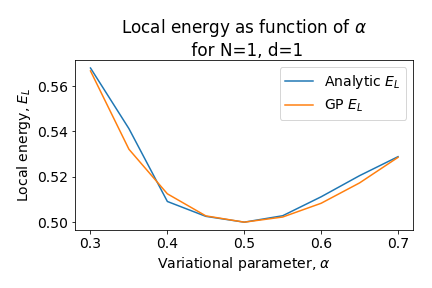
\includegraphics[width=0.6\linewidth, height=0.4\linewidth]{Check_alphas.png}
	\caption{Here we see how the local energy for non-interaction bosons in a spherical harmonic potential trap and the Gros-Pitaevskii calculated energy behaves as we vary the variational parameter $\alpha$ in the simplest case for one particle in one dimension. At our expected energy minimum for $\alpha=0.5$ we see that both curves are alike. \label{fig:check_alphas}}
\end{figure} 

In this same case we also look at how the acceptance rate, which is normalized by the number of MC step we use, behaves for the brute force Metropolis when we change the MC step length for the variational parameter $\alpha=0.5$. This behavior is observable in Figure \ref{fig:check_accept}. There we see that as the MC step length increases, the normalized acceptance rate of the proposed steps decline almost linearly.

\begin{figure}[htbp!]
	\centering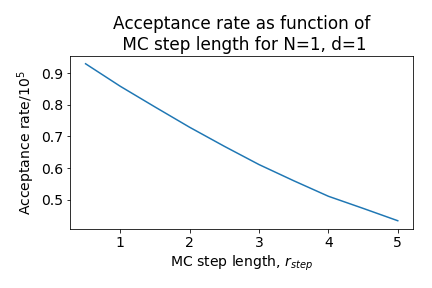
\includegraphics[width=0.6\linewidth, height=0.4\linewidth]{Check_accept.png}
	\caption{Here we see how the acceptance rate (normalized by the number of MC steps) of the proposed steps with brute force Metropolis for non-interaction bosons in a spherical harmonic potential trap behaves as we vary the MC step length $r_{\text{step}}$ in the simplest case for one particle in one dimension. \label{fig:check_accept}}
\end{figure} 

Next thing we wanted to test was the performance of the analytical expression of the local energy versus the numerical calculation of the kinetic energy with numerical derivation. In Table \ref{tab:analytic_vs_numeric} we see the results of the brute force Metropolis for both analytical and numerical ground state energy for $N=1,10,100,500$ particles in one, two and three dimensions. The parameters used are seen in the Method section \ref{subsubsect:Coding_non-int}. We also compare with the Gross-Pitaevskii calculation of the ground state energy (eq. \ref{eq:GP_derived}). From the table we see that the analytical expression gives slightly more accurate results in the ground state energy than the numerical derivation does compared with the GP calculated energies. The acceptance rates are also not very good, since they are so low. We also see that the error in the numerical energies get higher and higher as the number of particles and dimensions increases, but the accuracy is still very good. The main thing to notice is that the analytical expression becomes a lot faster as the number of particles and dimensions gets higher, which is why it is very beneficial to have an analytical expression to do the calculation with. That is why we use the analytical expressions in the rest of the calculations in this project.

\begin{table}[htbp!]
	\centering
	%\hspace{-1.0cm}
	\begin{tabular}{ |c|c|c|c|c|c|c|c|c| }
		\hline \rule{0pt}{13pt}
		N & d & $E_L^A$ & $A^A$ & $t^A[s]$ & $E_L^N$ & $A^N$ & $t^N[s]$ & $E_L^{GP}$ \\
		\hline \rule{0pt}{13pt}
		 & 1 & 0.5$\pm0.0$ & 0.513 & 0.1297 & 0.5$\pm2.02\cdot10^{-10}$ & 0.513 & 0.2645 & 0.5\\
		%\hline \rule{0pt}{13pt}
		1 & 2 & 1.0$\pm0.0$ & 0.512 & 0.1815 & 1.0$\pm3.00\cdot10^{-10}$ & 0.512 & 0.4134 & 1.0\\
		%\hline \rule{0pt}{13pt}
		 & 3 & 1.5$\pm0.0$ & 0.506 & 0.2473 & 1.5$\pm4.16\cdot10^{-10}$ & 0.506 & 0.6014 & 1.5\\
		\hline \rule{0pt}{13pt}
		 & 1 & 5.0$\pm0.0$ & 0.512 & 0.9724 & 5.0$\pm1.09\cdot10^{-9}$ & 0.512 & 5.0552 & 5.0\\
		%\hline \rule{0pt}{13pt}
		10 & 2 & 10.0$\pm0.0$ & 0.514 & 2.2701 & 10.0$\pm1.81\cdot10^{-9}$ & 0.514 & 15.657 & 10.0\\
		%\hline \rule{0pt}{13pt}
		& 3 & 15.0$\pm0.0$ & 0.506 & 2.9561 & 15.0$\pm5.84\cdot10^{-9}$ & 0.506 & 31.841 & 15.0\\
		\hline \rule{0pt}{13pt}
		 & 1 & 50.0$\pm0.0$ & 0.514 & 13.812 & 50.0$\pm1.28\cdot10^{-8}$ & 0.514 & 1062.6 & 50.0\\
		%\hline \rule{0pt}{13pt}
		100 & 2 & 100.0$\pm0.0$ & 0.516 & 23.779 & 100.0$\pm 2.64\cdot10^{-8}$ & 0.516 & $>>$1000 & 100.0\\
		%\hline \rule{0pt}{13pt}
		& 3 & 150.0$\pm0.0$ & 0.507 & 34.730 & 150.0$\pm4.28\cdot10^{-8}$ & 0.507 & $>>$1000 & 150.0\\
		\hline \rule{0pt}{13pt}
		 & 1 & 250.0$\pm0.0$ & 0.515 & 196.04 & 250.0$\pm9.31\cdot10^{-8}$ & 0.515 & $>>$1000 & 250.0\\
		%\hline \rule{0pt}{13pt}
		500 & 2 & 500.0$\pm0.0$ & 0.511 & 207.24 & 500.0$\pm2.05\cdot10^{-7}$ & 0.511 & $>>$1000 & 500.0\\
		%\hline \rule{0pt}{13pt}
		& 3 & 750.0$\pm0.0$ & 0.496 & 258.81 & 750.0$\pm6.37\cdot10^{-7}$ & 0.496 & $>>$1000 & 750.0\\
		\hline
	\end{tabular}	
	\caption{Table for the brute force Metropolis computation of the ground state energy ($E_L$), the acceptance rate ($A$) and the CPU time of the calculation in seconds ($t$) for 1-500 particles in 1-3 dimensions with the energy calculated from the Gross-Pitaevskii (GP) equation (\ref{eq:GP_derived}) and $\alpha=0.5$. For the analytical expression we use $i^A$, for the numerical calculation we use $i^N$ and for the GP calculated energy we use $E_L^{GP}$. See here that the analytical is slightly more accurate, and a lot faster than the numerical. \label{tab:analytic_vs_numeric}}
\end{table}

From these results we get an very small to non-existing error in the computation of the ground state energies. This is not a very realistic model to a quantum system, since there will always be some error to numerical computations. It is also not very realistic with a system like we are looking at without any interaction between the particles. But since our analytical expression for this simple non-interacting case is very simple and stable for the chosen parameters and natural units, our results are quite reasonable.

\subsection{Importance Sampling For Non-Interacting Bosons}
\label{subsect:Result_importance_non-int}
The next thing was to improve the brute force Metropolis by introducing a drift/quantum force and Importance sampling. Instead of a step length we needed a time step $\Delta t$. That is why we tested the normalized acceptance rate for this improved method by varying the time step $\Delta t\in[10^{-7},10]$. In Figure \ref{fig:check_timestep} we see how the acceptance ratio just barely decreases for very small $\Delta t$'s ($<10^{-4}$). Then after around $\Delta t=0.01$, it decreases quite rapidly. For $\Delta t<=0.001$, we get very good acceptance rates $A>=0.99257$. That is why we choose $\Delta t=0.001$ to be used for Importance sampling further one. This seems like a fitting choice, since the proposed step won't move too close to or too far away from the previous position.

\begin{figure}[htbp!]
	\centering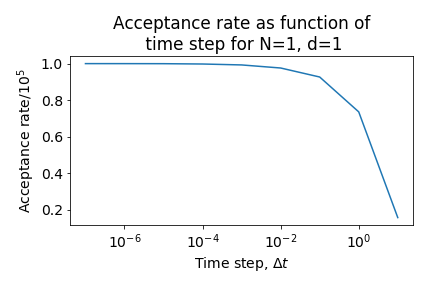
\includegraphics[width=0.6\linewidth, height=0.4\linewidth]{Check_timestep.png}
	\caption{Here we see how the acceptance rate (normalized by the number of MC steps) of the proposed steps with Importance sampling for non-interaction bosons in a spherical harmonic potential trap behaves as we vary the time step $\Delta t$ in the simplest case for one particle in one dimension. See that the acceptance ratio dropps rapidly after around $\Delta t=0.01$. \label{fig:check_timestep}}
\end{figure} 

Then we run the Importance sampling with $\Delta t=0.001$ where we compare the analytical to the numerical ground state energies for 1-500 particles in one, two and three dimensions. Here the drift force was computed analytically only to not slow down the program. In Table \ref{tab:imp_analytic_vs_numeric} we see the results of the same computation as in Table \ref{tab:analytic_vs_numeric} for the brute force Metropolis, but now for Importance sampling. Like for the brute force Metropolis, the analytical is supreme in CPU speed in comparison to the numerical derivation. When we compare the Importance sampling results in Table \ref{tab:imp_analytic_vs_numeric} to the results in Table \ref{tab:analytic_vs_numeric} obtained by the brute Metropolis, we see that the acceptance ratio now has increased from $\approx50$\% to $\approx0.99$\%. So the Importance sampling increases the acceptance ratio by a lot. So the Importance sampling method indeed makes better proposed steps towards the minimum local energy. The drawback with this sampling method is the speed. The CPU time of the Importance sampling becomes a lot higher than the brute Metropolis sampling. For the smaller systems with numerical derivation, we se the time with brute Metropolis is about half the time for Importance sampling. The reason for the increase in CPU time for Importance sampling, is the calculations of the drift force and Green's function. This is not the most interesting or realistic case, which is why we introduce interaction between the bosons next. From our results to save CPU time, we will use the analytical expression for the ground state energy and the brute Metropolis sampling for the rest of the project.

\begin{table}[htbp!]
	\centering
	%\hspace{-1.0cm}
	\begin{tabular}{ |c|c|c|c|c|c|c|c|c| }
		\hline \rule{0pt}{13pt}
		N & d & $E_L^A$ & $A^A$ & $t^A[s]$ & $E_L^N$ & $A^N$ & $t^N[s]$ & $E_L^{GP}$ \\
		\hline \rule{0pt}{13pt}
		& 1 & 0.5$\pm0.0$ & 0.993 & 0.4446 & 0.5$\pm2.59\cdot10^{-10}$ & 0.993 & 0.5361 & 0.5\\
		%\hline \rule{0pt}{13pt}
		1 & 2 & 1.0$\pm0.0$ & 0.989 & 0.6389 & 1.0$\pm5.15\cdot10^{-10}$ & 0.990 & 0.8500 & 1.0\\
		%\hline \rule{0pt}{13pt}
		& 3 & 1.5$\pm0.0$ & 0.986 & 1.1456 & 1.5$\pm5.77\cdot10^{-10}$ & 0.986 & 1.3629 & 1.5\\
		\hline \rule{0pt}{13pt}
		& 1 & 5.0$\pm0.0$ & 0.993 & 2.0850 & 5.0$\pm2.30\cdot10^{-9}$ & 0.993 & 10.307 & 5.0\\
		%\hline \rule{0pt}{13pt}
		10 & 2 & 10.0$\pm0.0$ & 0.989 & 4.4956 & 10.0$\pm2.56.\cdot10^{-9}$ & 0.989 & 29.992 & 10.0\\
		%\hline \rule{0pt}{13pt}
		& 3 & 15.0$\pm0.0$ & 0.986 & 5.9661 & 15.0$\pm5.41\cdot10^{-9}$ & 0.986 & 61.189 & 15.0\\
		\hline \rule{0pt}{13pt}
		& 1 & 50.0$\pm0.0$ & 0.994 & 76.677 & 50.0$\pm1.78\cdot10^{-8}$ & 0.994 & $>>$1000 & 50.0\\
		%\hline \rule{0pt}{13pt}
		100 & 2 & 100.0$\pm0.0$ & 0.991 & 158.25 & 100.0$\pm 3.29.\cdot10^{-8}$ & 0.991 & $>>$1000 & 100.0\\
		%\hline \rule{0pt}{13pt}
		& 3 & 150.0$\pm0.0$ & 0.988 & 255.65 & 150.0$\pm5.72\cdot10^{-8}$ & 0.988 & $>>$1000 & 150.0\\
		\hline \rule{0pt}{13pt}
		& 1 & 250.0$\pm0.0$ & 0.994 & 643.74 & 250.0$\pm1.03.\cdot10^{-7}$ & 0.994 & $>>$1000 & 250.0\\
		%\hline \rule{0pt}{13pt}
		500 & 2 & 500.0$\pm0.0$ & 0.992 & 718.86 & 500.0$\pm3.46.\cdot10^{-7}$ & 0.992 & $>>$1000 & 500.0\\
		%\hline \rule{0pt}{13pt}
		& 3 & 750.0$\pm0.0$ & 0.989 & 834.87 & 750.0$\pm6.85\cdot10^{-7}$ & 0.989 & $>>$1000 & 750.0\\
		\hline
	\end{tabular}	
	\caption{Table for the Importance sampling of the ground state energy ($E_L$), the acceptance rate ($A$) and the CPU time of the calculation in seconds ($t$) for 1-500 particles in 1-3 dimensions with the energy calculated from the Gross-Pitaevskii (GP) equation (\ref{eq:GP_derived}) and $\alpha=0.5$. For the analytical expression we use $i^A$, for the numerical calculation we use $i^N$ and for the GP calculated energy we use $E_L^{GP}$. As for brute Metropolis sampling, the analytical calculations are much faster than the numerical derivations. \label{tab:imp_analytic_vs_numeric}}
\end{table}

\subsection{Interacting Bosons}
\label{subsect:Results_int}
Then we turned to an elliptical potential trap for interacting bosons in three dimensions with $N=10,50,100$ particles. In this case we also get another trial wave function that contains the Jastrow factor with a hard-core sphere radius $a/a_{ho}=0.0043$, and the energies are now in units of $\hbar\omega_{ho}$. With the brute Metropolis we compute the local energies and their corresponding GP calculated energies, where we vary the variation parameter $\alpha\in[0.2,0.7]$. The reason we choose this range of variational parameters values is due to the similarities between the elliptical and spherical systems These results can be found in Table \ref{tab:alpha_int} and Figure \ref{fig:check_int_alpha}. From these results we notice also here an energy minimum around $\alpha=0.5$ as in the non-interacting system. We also see that the closer we are to the optimal variational parameter, the smaller the standard deviation/error in the energies become. As the number of particles increase, we see that our computed energies deviates (on average) a little more from the GP calculated energies. On average our computed energies has a tendency of overestimating the ground state energies, while the non-interacting energies gave more or less the exact energies as the GP calculated energies. A reason for this is that we considered the simpler solution of the GP equation which excluded the interaction between the bosons. The same figures as in Figure \ref{tab:alpha_int} for $N=10$ and $50$ can be found in the Figures folder at the GitHub repository \cite{GitHub}.

By looking at the computation of the local energies for non-interacting bosons in Table \ref{tab:analytic_vs_numeric} and for the interacting bosons in Table \ref{tab:alpha_int} for $N=10$ and $N=100$ particles in three dimensions, we see that the energies in the interacting system are higher than in the non-interacting system. So the interaction force between the bosons increase the ground state energy of the system. The energies also increase more and more in the interacting system compared to the respective energies in the non-interacting as the systems have a higher and higher number of particles in them. To inspect what the actual optimal variational parameters are, we will do a gradient descent method.

\begin{table}[htbp!]
	%\centering
	\hspace{-1.0cm}
	\begin{tabular}{ |c|c|c|c|c|c|c| }
		\hline \rule{0pt}{13pt}
		N & \multicolumn{2}{c|}{10} & \multicolumn{2}{c|}{50} & \multicolumn{2}{c|}{100}\\
		\hline \rule{0pt}{13pt}
		$\alpha$ & $E_L^{GP}[\hbar\omega_{ho}]$ & $E_L[\hbar\omega_{ho}]$ & $E_L^{GP}[\hbar\omega_{ho}]$ & $E_L[\hbar\omega_{ho}]$ & $E_L^{GP}[\hbar\omega_{ho}]$ & $E_L[\hbar\omega_{ho}]$ \\
		\hline \rule{0pt}{13pt}
		0.2 & 35.0061 & 34.7520$\pm0.0223$ & 175.031 & 172.283$\pm0.1759$ & 350.061 & 347.934$\pm0.2017$ \\
		\hline \rule{0pt}{13pt}
		0.3 & 27.3611 & 27.3888$\pm0.0116$ & 136.806 & 136.029$\pm0.0955$ & 273.611 & 274.833$\pm0.1299$ \\
		\hline \rule{0pt}{13pt}
		0.4 & 24.7457 & 24.7473$\pm0.0050$ & 123.729 & 124.623$\pm0.0389$ & 247.457 & 249.191$\pm0.04914$ \\
		\hline \rule{0pt}{13pt}
		0.5 & 24.1422 & 24.2348$\pm0.0002$ & 120.711 & 121.544$\pm0.0041$ & 241.422 & 242.585$\pm0.0094$ \\
		\hline \rule{0pt}{13pt}
		0.6 & 24.5445 & 24.6510$\pm0.0039$ & 122.723 & 124.141$\pm0.0262$ & 245.445 & 245.327$\pm0.0396$ \\
		\hline \rule{0pt}{13pt}
		0.7 & 25.5217 & 25.6830$\pm0.0074$ & 127.609 & 128.128$\pm0.0575$ & 255.217 & 252.210$\pm0.0805$ \\
		\hline
	\end{tabular}	
	\caption{Table for the computed local energies ($E_L$) and Gross-Pitaevskii energies ($E_L^{GP}$) for interacting bosons in an elliptical potential trap in three dimensions for $N=10,50,100$ particles. As for the non-interacting system. we can see a minimum in the energies for $\alpha=0.5$ here. The closer to the optimal variational parameter we are, the smaller are the standard deviation, or error, in the energies.  \label{tab:alpha_int}}
\end{table}

\begin{figure}[htbp!]
	\centering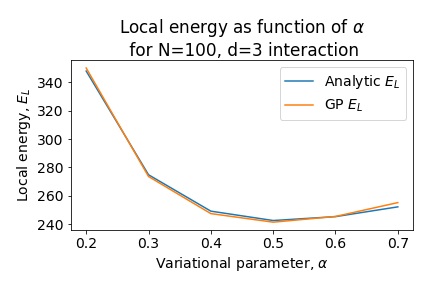
\includegraphics[width=0.6\linewidth, height=0.4\linewidth]{Check_alphas_int100.png}
	\caption{Here we see how the local energy for $N=100$ particles in a three dimensional elliptical potential trap for interacting bosons behaves as we vary the variational parameter $\alpha\in[0.2,0.7]$. See here that our computed energies are close to the Gross-Pitaevskii calculated energies. \label{fig:check_int_alpha}}
\end{figure} 

\subsection{Gradient Descent \& Optimal Parameter}
\label{subsect:Result_gradient}
To find the optimal variational parameter we introduced a (steepest) gradient descent method for both non-interacting and interacting bosons. This method finds the energy minimum of the system and for which $\alpha$ that happens. To do this we used $10^3$ number of MC steps with two separate initial guesses $\alpha=0.45, 0.55$ for each of the $N=10,50,100$ particles in three dimensions. These results are given in Table \ref{tab:gradient}. There we see the optimal $\alpha$ we got for the two initial guesses, separately, and the mean of the two to get the optimal parameter for that set of particles. For the non-interacting case, this was not very interesting to look at, since we just got the analytically calculated parameter $\alpha=0.5$ as we expected. For the interaction, we see that the optimal parameter increases a little as the number of particles increase. A thing to notice about the gradient descent method, is that it is very sensitive to where we choose our initial guesses as well as what our factor $\lambda$ is chosen to be. That is why a adaptive gradient descent method might be better since it adapts the constant factor as the method iterates.

With the optimal variational parameters we did the VMC computation again to get the ground state energies for the same cases. These results are found in Table \ref{tab:optimal_alpha_grad}. The standard deviation/error in the ground state energies for the interacting bosons are not very large. We would actually expect the errors to be bigger since the numerical data are not fully uncorrelated. That is why we want to do a statistical analysis to get more realistic errors.

\begin{table}[htbp!]
	\centering
	%\hspace{-1.0cm}
	\begin{tabular}{ |c|c|c|c|c|c|c| }
		\hline \rule{0pt}{13pt}
		\text{System} & \multicolumn{3}{c|}{\text{Non-interacting}}  & \multicolumn{3}{c|}{\text{Interacting}}\\
		\hline \rule{0pt}{13pt}
		N & $\alpha_{\text{guess, 0.45}}$ & $\alpha_{\text{guess, 0.55}}$ & $\alpha_{\text{optimal}}$ & $\alpha_{\text{guess, 0.45}}$ & $\alpha_{\text{guess, 0.55}}$ & $\alpha_{\text{optimal}}$  \\
		\hline \rule{0pt}{13pt}
		10 & 0.5 & 0.5 & 0.5 & 0.495842 & 0.519972 & 0.507907 \\
		\hline \rule{0pt}{13pt}
		50 & 0.5 & 0.5 & 0.5 & 0.503473 & 0.518021 & 0.510747 \\
		\hline \rule{0pt}{13pt}
		100 & 0.5 & 0.5 & 0.5 & 0.505201 & 0.520115 & 0.512658 \\
		\hline
	\end{tabular}	
	\caption{Table for the (steepest) gradient descent method for finding the optimal variational parameter $\alpha_{\text{optimal}}$ for non-interacting and interacting systems in three dimensions and for $N=10,50,100$ particles. $\alpha_{\text{optimal}}$ is the average parameter of the two optimal $\alpha$'s we get from the two guesses $\alpha=0.45,0.55$ for that corresponding particle. See that for non-interaction we get as we expected $\alpha=0.5$. For interaction the optimal $\alpha$ increases as the number of particles increases, but is still close to the optimal $\alpha$ for the non-interacting case. \label{tab:gradient}}
\end{table}

\begin{table}[htbp!]
	\centering
	%\hspace{-1.0cm}
	\begin{tabular}{ |c|c|c|c|c| }
		\hline \rule{0pt}{13pt}
		\text{System} & \multicolumn{2}{c|}{\text{Non-interacting}}  & \multicolumn{2}{c|}{\text{Interacting}} \\
		\hline \rule{0pt}{13pt}
		N &  $\alpha_{\text{optimal}}$ & $E_L[\hbar\omega_{ho}]$ & $\alpha_{\text{optimal}}$ & $E_L[\hbar\omega_{ho}]$ \\
		\hline \rule{0pt}{13pt}
		10 & 0.5 & 15 & 0.507907 & 24.242$\pm3.226\cdot10^{-4}$ \\
		\hline \rule{0pt}{13pt}
		50 & 0.5 & 75 & 0.510747 & 121.592$\pm1.787\cdot10^{-3}$ \\
		\hline \rule{0pt}{13pt}
		100 & 0.5 & 150 & 0.512658 & 242.332$\pm2.306\cdot10^{-3}$ \\
		\hline
	\end{tabular}	
	\caption{Table for the brute Metropolis computation of the ground state energies with the optimal variational parameters $\alpha_{\text{optimal}}$ found through the gradient descent method for both non-interacting and interacting bosons for $N=10,50,100$ particles. \label{tab:optimal_alpha_grad}}
\end{table}

\subsection{Statistical Analysis}
\label{subsect:Result_analysis}
With the optimal variational parameters found for the non-interacting and interacting systems from the gradient descent method, we did a statistical analysis by using the blocking method by \citet{jonsson2018standard}. Since the non-interacting system only has $\alpha_{\text{optimal}}=0.5$ there was no need to do an improvement on the statistical error, since there is no error to improve upon. So for the interacting system we ran the VMC using the optimal $\alpha_{\text{optimal}}$'s in Table \ref{tab:optimal_alpha_grad}, where we exported all the local energies for each MC cycle to a file. Then we did the statistical analysis on these energies to get the ground state energies with the improved errors we see in Table \ref{tab:blocking_energies}. By comparing the standard deviation in the energies in Table \ref{tab:optimal_alpha_grad} and Table \ref{tab:blocking_energies}, we see that the energies after applying the blocking method has a higher standard deviation. This seems more correct, since the blocking methods has taken into consideration the correlation between the numerically produced data.

\begin{table}[htbp!]
	\centering
	%\hspace{-1.0cm}
	\begin{tabular}{ |c|c|c|c| }
		\hline \rule{0pt}{13pt}
		\text{System} &  \multicolumn{2}{c|}{\text{Interacting}} & \text{GP eq.}\\
		\hline \rule{0pt}{13pt}
		N & $\alpha_{\text{optimal}}$ & $E_L[\hbar\omega_{ho}]$ & $E_L^{GP}[\hbar\omega_{ho}]$\\
		\hline \rule{0pt}{13pt}
		10 & 0.507907 & 24.242$\pm0.0025$ & 24.1427 \\
		\hline \rule{0pt}{13pt}
		50 & 0.510747 & 121.592$\pm0.0569$ & 120.926 \\
		\hline \rule{0pt}{13pt}
		100 & 0.512658 & 242.332$\pm0.0999$ & 241.658 \\
		\hline
	\end{tabular}	
	\caption{Table for the ground state energies with their respective optimal variational parameter $\alpha_{\text{optimal}}$ for the $N$-particles in three dimensions after using the blocking method to improve the standard deviation in the energies. See here that the error in th energies have increased in comparison to values in Table \ref{tab:optimal_alpha_grad}. \label{tab:blocking_energies}}
\end{table}

\subsection{One-Body Density}
\label{subsect:Result_onbody}
Then we looked at the one-body density of the systems which was computed by sampling the radial distance for each particle, with their respective optimal variational parameter, in each of the MC cycles after calibrating into bins and normalization of the probability. This distribution of particles is used to look at the effect the particle-interaction/Jastrow factor has on the system. This is shown in Figure \ref{fig:onebody}. There we see the one-body density, or the probability of bosons being at a radial distance from each other in units of $r/a_{ho}$, for 100 particles in three dimensions. We can barely see that the probability curve with the Jastrow factor is not so steep as without the factor after we have reached the most likely radial distance. Similar figures like Figure \ref{fig:onebody} for 10 and 50 particles can be seen in the Figures folder at the GitHub repository \cite{GitHub}.

\begin{figure}[htbp!]
	\centering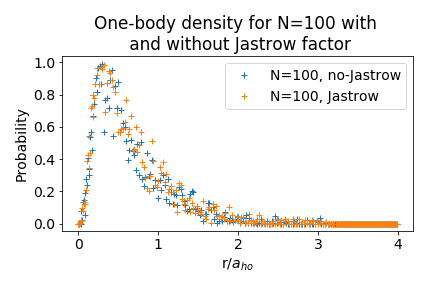
\includegraphics[width=0.6\linewidth, height=0.4\linewidth]{onebody_N_100.png}
	\caption{Here we see the one-body density of bosons in an elliptical harmonic oscillator trap with and without the Jastrow factor. We can just see that with the factor, the curve reaches zero later or further away from each other than without the factor. \label{fig:onebody}}
\end{figure} 

\section{Conclusion}
\label{sect:Conclusion}
In this project we have made a variational Monte Carlo solver where our goal was to compute the ground state energies of quantum systems containing non-interacting and interacting bosons in spherical and elliptical harmonic oscillator traps. To do these calculations we have both analytically and numerically calculated the ground state energies and used both a brute force Metropolis and an improved Metropolis-Hastings (Importance) sampling to do the computation for $N\in[1,500]$ particles in one, two and three dimensions. These energies were benchmarked against the Gross-Pitaevskii calculated energies. The Importance sampling proved to give higher acceptance rates, but was slower than the brute Metropolis. For the energy calculation we found that the analytical calculation was superior in CPU time against the numerically calculated kinetic energies. That is why an analytical expression is preferred over the numerical calculation. In many other cases, we might not be so lucky that we can find an analytical expression. Then we compared the non-interacting system in a spherical trap to an interacting system in an elliptical trap. For the non-interacting system we got spot on ground state energies compared with the GP energies, while for interaction we got close to the GP calculated energies. We also came to a conclusion that the interacting force between the bosons increased the energies in the systems more and more as the number of particles in the system increased, in comparison to the respective energies for non-interacting bosons. Then we used a steepest gradient descent method to find the optimal variational parameter for each set of particles in three dimensions. These was as expected where we got $\alpha=0.5$ for all particle cases in the non-interacting case. For interacting bosons we got optimal parameters close to 0.5. As the number of particles increased, the more increased the optimal parameter also. Then we improved the statistical errors in the ground state energies by using a blocking method which takes into consideration the correlation in the numerically produced data. The last thing we did was to study the Jastrow factor dependency on the system. There we got that the Jastrow factor increased the system energies and that the probability was higher at a distance further away from the bosons, so it can be interpreted as an interaction.

For future work we could try to parallelize the code to make it run faster. Another future aspect could be to study systems of fermions in stead of only bosons, which is a simpler system since they only have integer of spins. We could also try to implement machine learning and neural networks in the ground state energy computations.

\appendix
\section*{Appendix:}
\section{Gross-Pitaevskii Equation}
\label{appendix:GP_eq}
For a non-interacting system with $a=0$ for N particles we use with a normalized trial wave function 
\begin{align}
\label{eq:norm_WF_T}
\Psi_T&=\left(\frac{2\alpha}{\pi}\right)^{\frac{3N}{4}}\beta^{\frac{N}{4}}\prod_{i}e^{-\alpha(x_i^2+y_i^2+\beta z_i^2)}\\
\nabla\Psi_T&=\left(\frac{2\alpha}{\pi}\right)^{\frac{3N}{4}}\beta^{\frac{N}{4}}\prod_{i}e^{-\alpha(r_i^2)}\cdot\sum_i(-2\alpha(x_i\textbf{e}_x+y_i\textbf{e}_y+\beta z_i\textbf{e}_z))
\end{align}
The GP equation (\ref{eq:GP_eq}) can then be rewritten to
\begin{align*}
E_{GP}[\Psi_T]&=\sum_i\int(2\alpha^2+\frac{1}{2})(x_i^2+y_i^2+\beta z_i^2)|\Psi_T|^2d\textbf{r}\nonumber\\
&=(2\alpha^2+\frac{1}{2})\left(\frac{2\alpha}{\pi}\right)^{\frac{3N}{2}}\beta^{\frac{N}{2}}\frac{N}{4\alpha}(\beta+2)\left(\frac{\pi}{2\alpha}\right)^{\frac{3N}{2}}\beta^{-\frac{N}{2}}\nonumber\\
&=\frac{N}{2}\left(\alpha+\frac{1}{4\alpha}\right)(\beta+2).
\end{align*}

\section{Non-Interacting Optimal Parameter}
\label{appendix:Optimal_alpha}
To find the optimal $\alpha$-parameter for non-interacting bosons for N particles in three dimensions with $\omega=1$ we take the partial derivative of the expected local energy in equation \ref{eq:local_E_nonint} with respect to the variational parameter:
\[\frac{\partial \langle E_L\rangle}{\partial \alpha}=0\]
\begin{align*}
\frac{\partial}{\partial \alpha}\left(\alpha dN+(-2\alpha^2+\frac{1}{2})\sum_{i=1}^{N}r_i^2\right)&=\frac{\partial}{\partial \alpha}\left(\alpha dN-\alpha^2dN+\frac{dN}{4}\right)=(dN-2\alpha dN)=0\\
\Rightarrow 2\alpha dN&=dN\\
\Rightarrow \alpha&=0.5
\end{align*}

\section{Derivation of The Interacting Laplacian}
\label{appendix:Laplacian}
Derivation of the gradient of the trial wave function for interaction between bosons is: (Note that we have to change the indices since they are different)
\begin{align}
\label{eq:grad_int}
\nabla_k\Psi_T(\textbf{r})&=\nabla_k\left[\prod_i \phi(\textbf{r}_i)
\exp\left(\sum_{j<m}u(r_{jm})\right)\right]\nonumber\\
&=\nabla_k\phi(\textbf{r}_k)\left[\prod_{i\neq k}\phi(\textbf{r}_i)\right] \exp\left(\sum_{j<m}u(r_{jm})\right) +\left[\prod_{i}\phi(\textbf{r}_i)\right]\nabla_k\left[\exp\left(\sum_{j<m}u(r_{jm})\right)\right]\nonumber\\
&=\nabla_k\phi(\textbf{r}_k)\left[\prod_{i\neq k}\phi(\textbf{r}_i)\right] \exp\left(\sum_{j<m}u(r_{jm})\right) +\left[\prod_{i}\phi(\textbf{r}_i)\right]\exp\left(\sum_{j<m}u(r_{jm})\right)\sum_{l\neq k}\nabla_k u(r_{kl})\nonumber\\
&=\frac{\nabla_k\phi(\textbf{r}_k)}{\phi(\textbf{r}_k)}\Psi_T(\textbf{r})+\Psi_T(\textbf{r})\sum_{l\neq k}\nabla_k u(r_{kl})
\end{align}

Derivation of the Laplacian of the interacting trial wave function for a particle $k$:
\begin{align*}
\nabla_k^2\Psi_T(\textbf{r})&=\nabla_k^2\phi(\textbf{r}_k)\prod_{i\neq k}\phi(\textbf{r}_i)\exp\left(\sum_{j<m}u(r_{jm})\right)\\
&+ 2\nabla_k\phi(\textbf{r}_k)\prod_{i\neq k}\phi(\textbf{r}_i)\exp\left(\sum_{j<m}u(r_{jm})\right)\sum_{j\neq k}\nabla_ku(r_{kj})\\
&+ \prod_{i}\phi(\textbf{r}_i)\exp\left(\sum_{j<m}u(r_{jm})\right)\sum_{j\neq k}\nabla_ku(r_{kj})\sum_{i\neq k}\nabla_ku(r_{ki})\\
&+ \prod_{i}\phi(\textbf{r}_i)\exp\left(\sum_{j<m}u(r_{jm})\right)\sum_{j\neq k}\nabla_k^2u(r_{kj})
\end{align*}
The Laplacian divided by the trial wave function becomes:
\begin{align*}
\frac{\nabla_k^2\Psi_T(\textbf{r})}{\Psi_T(\textbf{r})}=\frac{\nabla_k^2\phi(\textbf{r}_k)}{\phi(\textbf{r}_k)}+2\frac{\nabla_k\phi(\textbf{r}_k)}{\phi(\textbf{r}_k)}\sum_{j\neq k}\nabla_ku(r_{kj})+\sum_{j\neq k}\nabla_ku(r_{kj})\sum_{i\neq k}\nabla_ku(r_{ki})+\sum_{j\neq k}\nabla_k^2u(r_{kj})
\end{align*}
Need now to compute $\nabla_k u(r_{kj})$ and $\nabla_k^2u(r_{kj})$:
\begin{align*}
\nabla_ku(r_{kj})&=u^{\prime}(r_{kj})\nabla_k r_{kj}=u^{\prime}(r_{kj})\nabla_k\sqrt{(\textbf{r}_k-\textbf{r}_j)^2}=u^{\prime}(r_{kj})\frac{\textbf{r}_k-\textbf{r}_j}{\sqrt{(\textbf{r}_k-\textbf{r}_j)^2}}=u^{\prime}(r_{kj})\frac{\Delta\textbf{r}_{kj}}{r_{kj}}\\
\nabla_k^2u(r_{kj})&=u^{\prime\prime}(r_{kj})\frac{\Delta\textbf{r}_{kj}}{r_{kj}}+u^{\prime}(r_{kj})\nabla_k\left(\frac{\Delta\textbf{r}_{kj}}{r_{kj}}\right)
=u^{\prime\prime}(r_{kj})+\frac{2}{r_{kj}}u^{\prime}(r_{kj})
\end{align*}
\begin{align*}
\Rightarrow \frac{\nabla_k^2\Psi_T(\textbf{r})}{\Psi_T(\textbf{r})}&= \frac{\nabla_k^2\phi(\textbf{r}_k)}{\phi(\textbf{r}_k)}+2\frac{\nabla_k\phi(\textbf{r}_k)}{\phi(\textbf{r}_k)}\left(\sum_{j\neq k}u^{\prime}(r_{kj})\frac{\Delta\textbf{r}_{kj}}{r_{kj}}\right)+\sum_{i,j\neq k}\frac{\Delta \textbf{r}_{ki}\Delta \textbf{r}_{kj}}{r_{ki}r_{kj}}u^{\prime}(r_{ki})u^{\prime}(r_{kj})\\
&+\sum_{j\neq k}\left(u^{\prime\prime}(r_{kj})+\frac{d-1}{r_{kj}}u^{\prime}(r_{kj})\right)
\end{align*}
For the single-particle function with interaction we evaluate the gradient and the Laplacian:
\begin{align}
\label{eq:eval_grad_one}
\frac{\nabla_k\phi(\textbf{r}_k)}{\phi(\textbf{r}_k)}&=-2\alpha(x_k\textbf{e}_x+y_k\textbf{e}_y+\beta z_k\textbf{e}_z)\\
\label{eq:eval_laplacian_one}
\frac{\nabla_k^2\phi(\textbf{r}_k)}{\phi(\textbf{r}_k)}&=-2\alpha(d-1+\beta)+4\alpha^2(x_k^2+y_k^2+\beta^2z_k^2)
\end{align}
Then the same for the correlation function (eq. \ref{eq:Jastrow}):
\begin{align}
\label{eq:eval_grad_int}
u^{\prime}(r_{kj})&=\frac{\partial u(r_{kj})}{\partial r_{kj}}=\frac{a}{r_{kj}(r_{kj}-a)}\\
\label{eq:eval_laplacian_int}
u^{\prime\prime}(r_{kj})&=\frac{\partial^2 u(r_{kj})}{\partial r_{kj}^2}=\frac{a^2-2ar_{kj}}{r_{kj}^2(r_{kj}-a)^2}
\end{align}

\section{Derivation of Interaction Local Energy}
\label{appendix:local_E}
Inserting the gradient and Laplacian expressions for the single-particle function and the correlation function (eq. \ref{eq:eval_grad_one} to \ref{eq:eval_laplacian_int}) into the Laplacian divided by the trial wave function:
\begin{align}
\label{eq:H_int_deriv}
\frac{\nabla_k^2\Psi_T(\textbf{r})}{\Psi_T(\textbf{r})}&= \left(-2\alpha(d-1+\beta)+4\alpha^2(x_k^2+y_k^2+\beta^2z_k^2)\right)\nonumber\\
&+\left(-4\alpha(x_k\textbf{e}_x+y_k\textbf{e}_y+\beta z_k\textbf{e}_z)\right)\left(\sum_{j\neq k}\frac{a}{(r_{kj}-a)}\frac{\Delta\textbf{r}_{kj}}{r_{kj}^2}\right)\nonumber\\
&+\sum_{j\neq k}\left(\frac{a^2-2ar_{kj}}{r_{kj}^2(r_{kj}-a)^2}+\frac{d-1}{r_{kj}^2}\frac{a}{(r_{kj}-a)}\right)\nonumber\\
&+\sum_{i,j\neq k}\frac{\Delta \textbf{r}_{kj}\Delta \textbf{r}_{ki}}{r_{kj}^2r_{ki}^2}\frac{a^2}{(r_{kj}-a)(r_{kji}-a)}
\end{align}
The local energy for the interacting bosons:
\begin{align}
\label{eq:local_E_deriv}
E_L(\textbf{r})&=\sum_k^N\left(\frac{-\hbar^2}{2m}\frac{\nabla_k^2\Psi_T(\textbf{r})}{\Psi_T(\textbf{r})}+\frac{1}{\Psi_T(\mathbf{r})}V_{\text{ext}}(\textbf{r}_k)\Psi_T(\mathbf{r})\right)+\frac{1}{\Psi_T(\mathbf{r})}\sum_{j<k}^{N}V_{\text{int}}(\textbf{r}_j,\textbf{r}_k)\Psi_T(\mathbf{r})\nonumber\\
&=-\frac{\hbar^2}{2m}\sum_k^N\frac{\nabla_k^2\Psi_T(\textbf{r})}{\Psi_T(\textbf{r})}
+\frac{1}{2}m\sum_k^N[\omega^2(x_k^2+y_k^2) + \omega_z^2z_k^2]
+\sum_{j<k}^{N}V_{\text{int}}(\textbf{r}_j,\textbf{r}_k)
\end{align}

\bibliographystyle{plainnat}
\bibliography{myrefs}
\end{document}
